
% Copyright (c) 2015 - 2020 Mario Mlačak, mmlacak@gmail.com
% Licensed and published as Public Domain work.

% Conquest of Tlalocan chapter ========================================
\chapter*{Conquest of Tlalocan}
\addcontentsline{toc}{chapter}{Conquest of Tlalocan}

\begin{flushright}
\parbox{0.8\textwidth}{
\emph{The human mind is inspired enough when it comes to inventing
horrors; it is when it tries to invent a Heaven that it shows itself
cloddish. \\
\hspace*{\fill}{\textperiodcentered \textperiodcentered \textperiodcentered \hspace*{0.2em} Evelyn Waugh} } }
\end{flushright}

\noindent
Conquest of Tlalocan is chess variant which is played on 24 x 24 board,
with bright red and cyan fields, and dark red and light green pieces.
Star colors are bright red and bright blue. In algebraic notation, columns
are enumerated from 'a' to 'x', and rows are enumerated from '1' to '24'.
A new piece is introduced, Shaman.

\clearpage % ..........................................................
% Shaman **************************************************************

\section*{Shaman}
\addcontentsline{toc}{section}{Shaman}

\noindent
\begin{wrapfigure}[11]{l}{0.4\textwidth}
\centering
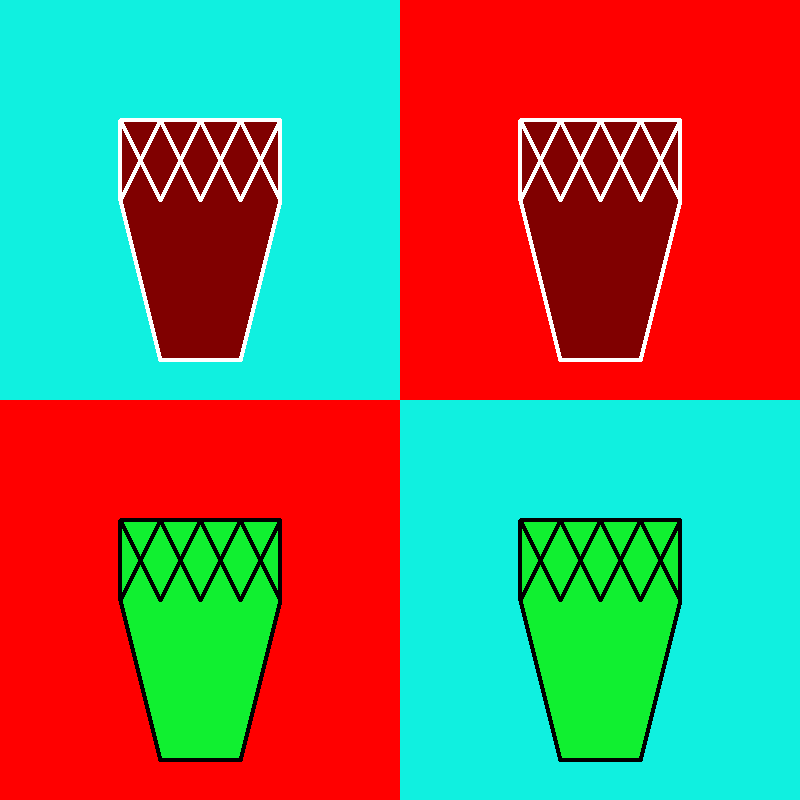
\includegraphics[width=0.4\textwidth, keepaspectratio=true]{pieces/14_shaman.png}
\caption{Shaman}
\label{fig:14_shaman}
\end{wrapfigure}
Shaman moves like sort-of cross between Knight and long-jump Unicorn,
where one figure provides step-fields, and the other capture-fields.

For light Shaman, step-fields are provided by the Knight, while capture-fields
are provided by long-range Unicorn. For dark Shaman, it's the opposite.

Shaman can continue it's jumpy movement in chosen direction; over step-fields
if they're empty, over capture-fields as long as it's capturing opponent's
pieces. Shaman can't change direction once started moving.

Shaman can activate both Wave and Pyramid on its' capture-fields, while only
Wave can be activated on step-fields. In all cases, activation ends Shaman's
ply.

% \vspace*{0.05\textheight}
\noindent
\begin{wrapfigure}{l}{0.4\textwidth}
\centering
\includegraphics[width=0.4\textwidth, keepaspectratio=true]{pieces/star/18_conquest_of_tlalocan.png}
\caption{Star}
\label{fig:star/18_conquest_of_tlalocan}
\end{wrapfigure}
Alternative move for Shaman is a trance-journey.

Shaman symbol in algebraic notation is 'H', to avoid confusion with Serpent.

Star colors in this variant are presented on the left.

\clearpage % ..........................................................
% Movement ------------------------------------------------------------

\subsection*{Movement}
\addcontentsline{toc}{subsection}{Movement}

\noindent
\begin{figure}[!h]
% \begin{figure}[!t]
\includegraphics[width=1.0\textwidth, keepaspectratio=true]{examples/18_cot/scn_cot_01_shaman_movement.png}
\caption{Shaman's movement}
\label{fig:scn_cot_01_shaman_movement}
% \centering
\end{figure}

For this variant examples are rendered in B\&W to improve legibility.
Here, step-fields are marked green, while capture-fields are marked blue.
Note, movement of Shaman does not depend on color of field on which it
stands, only on color of the piece itself.

\clearpage % ..........................................................

\noindent
\begin{figure}[!h]
% \begin{figure}[!t]
\includegraphics[width=1.0\textwidth, keepaspectratio=true]{examples/18_cot/scn_cot_02_light_shaman_step_ply.png}
\caption{Light Shaman's step-ply}
\label{fig:scn_cot_02_light_shaman_step_ply}
% \centering
\end{figure}

Once initial step-direction is chosen, light Shaman has to follow it,
and so moves similar to Pegasus. Unlike Pegasus, Shaman can't capture
opponent's pieces on step-fields, nor activate Pyramid. Wave on step-field
can be activated, and would continue to move as Shaman (and Pegasus)
would. Again, once direction is chosen, it cannot be changed, neither
in other step- nor capture-direction, even if opponent's piece is present
on capture-field.

\clearpage % ..........................................................

\noindent
\begin{figure}[!h]
% \begin{figure}[!t]
\includegraphics[width=1.0\textwidth, keepaspectratio=true]{examples/18_cot/scn_cot_03_light_shaman_capture_ply.png}
\caption{Light Shaman's capture-ply}
\label{fig:scn_cot_03_light_shaman_capture_ply}
% \centering
\end{figure}

Capture-ply can only be started with immediate capture, after which Shaman
can continue its' movement as long as it's keep capturing opponent's pieces
in the same direction. Empty capture-fields cannot be oversteped, any piece
at a distance is out of reach. Again, once started capturing, Shaman cannot
change it's heading, neither in other step- nor capture-direction. Shaman
can also activate Pyramid or Wave on capture-field, thus ending it's ply.

\clearpage % ..........................................................

\noindent
\begin{figure}[!h]
% \begin{figure}[!t]
\includegraphics[width=1.0\textwidth, keepaspectratio=true]{examples/18_cot/scn_cot_04_dark_shaman_step_ply.png}
\caption{Dark Shaman's step-ply}
\label{fig:scn_cot_04_dark_shaman_step_ply}
% \centering
\end{figure}

Dark Shaman's step-ply is the same as light Shaman's, except it steps like a
long-jump Unicorn, in chosen direction. Shaman can't capture opponent's pieces
on step-fields, nor activate Pyramid. Wave on step-field can be activated, and
would continue to move as dark Shaman would. Again, once direction is chosen,
it cannot be changed, neither in other step- nor capture-direction, even if
opponent's piece is present on capture-field.

\clearpage % ..........................................................

\noindent
\begin{figure}[!h]
% \begin{figure}[!t]
\includegraphics[width=1.0\textwidth, keepaspectratio=true]{examples/18_cot/scn_cot_05_dark_shaman_capture_ply.png}
\caption{Dark Shaman's capture-ply}
\label{fig:scn_cot_05_dark_shaman_capture_ply}
% \centering
\end{figure}

Dark Shaman's capture-ply is the same as light Shaman's, except it captures like
Pegasus, in chosen direction. Capture-ply can be initiated with immediate capture,
after which Shaman can continue capturing opponent's pieces, in the same direction,
if there is no empty capture-field in-between. While capturing, Shaman cannot change
it's heading to any other direction. Shaman can also activate Pyramid or Wave on
capture-field, thus ending it's ply.

\clearpage % ..........................................................

\subsubsection*{Activating Wave}
\addcontentsline{toc}{subsubsection}{Activating Wave}

\noindent
\begin{figure}[!h]
% \begin{figure}[!t]
\includegraphics[width=1.0\textwidth, keepaspectratio=true]{examples/18_cot/scn_cot_06_wave_activated.png}
\caption{Shaman activated Wave}
\label{fig:scn_cot_06_wave_activated}
% \centering
\end{figure}

Activated Wave moves the same as activating piece in the moment of activation.
So, if activated on, say,
\hyperref[fig:scn_cot_03_light_shaman_capture_ply]{light Shaman's capture-field},
Wave would move too as long-range Unicorn, in this case with momentum of 3.

% ------------------------------------------------------------ Movement
\clearpage % ..........................................................
% Trance-journey ------------------------------------------------------

\subsection*{Trance-journey}
\addcontentsline{toc}{subsection}{Trance-journey}

\noindent
\begin{wrapfigure}[13]{l}{0.4\textwidth} % [11]
\centering
\includegraphics[width=0.375\textwidth, keepaspectratio=true]{examples/18_cot/scn_cot_07_trance_journey_init.png}
\caption{Start}
\label{fig:scn_cot_07_trance_journey_init}
\end{wrapfigure}
Trance-journey can be started by activating a Shaman, if at least one other
Shaman precedes it in a cascade. Colors of Shamans do not need to match.

Shaman taking on trance-journey is called entranced Shaman (in this example,
dark Shaman 3), while the one immediately preceding it is called entrancing
Shaman (here, the light Shaman 2).

Whether entrancing Shaman started a cascade or was activated is not relevant,
mere existance of two Shamans in a cascade is enough to grant trance-journey
option.

Trance-journey can be undertaken even if entranced Shaman received no momentum.
Length of trance-journey is not limited by received momentum.

Note, trance-journey can be undertaken, but is not obligatory. Light Shaman 2
could also undertake trance-journey, in which case entrancing Shaman would be
light Shaman 1.
Had it received any momentum, dark Shaman 3 could also move just as
\hyperref[fig:scn_cot_04_dark_shaman_step_ply]{a long-jump Unicorn}.

\clearpage % ..........................................................

% \vspace*{0.05\textheight}
\subsubsection*{Movement}
\addcontentsline{toc}{subsubsection}{Movement}

\noindent
\begin{wrapfigure}[10]{l}{0.4\textwidth} % [11]
\centering
\includegraphics[width=0.375\textwidth, keepaspectratio=true]{examples/18_cot/scn_cot_08_knight_directions.png}
\caption{Knight directions}
\label{fig:scn_cot_08_knight_directions}
\end{wrapfigure}
If we look from Knight's position forward, then one direction would be to
the left, and the other to the right (here, dark Knight on the right).

Now, we can take all left steps, and arrange them so that step-field of one
Knight ends up on starting field of another, with red arrow ending at field S.

% \clearpage % ..........................................................

\vspace*{0.10\textheight}
\noindent
\begin{wrapfigure}[12]{l}{0.4\textwidth} % [11]
\centering
\includegraphics[width=0.375\textwidth, keepaspectratio=true]{examples/18_cot/scn_cot_09_stop_sign_pattern.png}
\caption{Stop sign pattern}
\label{fig:scn_cot_09_stop_sign_pattern}
\end{wrapfigure}
Result is a stop sign pattern. It can be traversed by Knight in 4 left-only
steps (moves), starting from field S.

Each step starts with horizontal or vertical leg, and finishes with diagonal
leg. Legs are referred to by relative position of its' end point.

So, starting step (green) has right and up-right legs, while last step (red)
has down and down-right legs.

\clearpage % ..........................................................

% \vspace*{0.05\textheight}
\noindent
\begin{wrapfigure}{l}{0.4\textwidth} % [11]
\centering
\includegraphics[width=0.375\textwidth, keepaspectratio=true]{examples/18_cot/scn_cot_10_stop_sign_pattern_unwind.png}
\caption{Stop sign pattern unwinded}
\label{fig:scn_cot_10_stop_sign_pattern_unwind}
\end{wrapfigure}
To untangle this pattern, after each step both legs (horizontal or vertical,
and diagonal) gets longer by 1.

So, starting step (green) has both legs with length of 1. Next step (blue)
has up and up-left legs both with length of 2, third step (dark grey) has
legs' lengths of 3, and so on. Pattern never ends.

Complementary to pattern starting with right leg (in the example to the
left), there is also symetrical pattern starting with left leg, i.e.
rotated by 180$^{\circ}$. % degrees.

\clearpage % ..........................................................

\noindent
\begin{figure}[!h]
% \begin{figure}[!t]
\includegraphics[width=1.0\textwidth, keepaspectratio=true]{examples/18_cot/scn_cot_12_light_shaman_trance_journey.png}
\caption{Light Shaman trance-journey}
\label{fig:scn_cot_12_light_shaman_trance_journey}
% \centering
\end{figure}

Together, left (blue) and right (green) hand pattern make a complete movement
pattern of light Shaman. After choosing direction (color), light Shaman
continues its' movement from starting position outwards. Shaman can stop at
any step-field on chosen colored pattern, even if previous step-fields lay
outside of a chessboard. If Shaman stops on a step-field outside of a
chessboard, it's removed from further game play, as if it has been captured
by the opponent.

\clearpage % ..........................................................

\noindent
\begin{figure}[!h]
% \begin{figure}[!t]
\includegraphics[width=1.0\textwidth, keepaspectratio=true]{examples/18_cot/scn_cot_13_light_shaman_trance_journey_offset.png}
\caption{Light Shaman trance-journey with offset}
\label{fig:scn_cot_13_light_shaman_trance_journey_offset}
% \centering
\end{figure}

\hyperref[fig:scn_hd_04_centaur_off_board]{Again},
light grey fields are virtual fields extending existing chessboard.

Based on a previous example, direction chosen was right (green) hand pattern.
If destination is field 5, traversed step-fields are 1, 2, virtual field 3,
fields 4 and 5, in that order. All other (step-)fields are not affected.

\clearpage % ..........................................................

\noindent
\begin{figure}[!h]
% \begin{figure}[!t]
\includegraphics[width=1.0\textwidth, keepaspectratio=true]{examples/18_cot/scn_cot_14_dark_shaman_trance_journey.png}
\caption{Dark Shaman trance-journey}
\label{fig:scn_cot_14_dark_shaman_trance_journey}
% \centering
\end{figure}

Dark Shaman's pattern is the same as light one's, except: \\
- complete pattern consists of up (green) and down (blue) hand pattern \\
- dark Shaman starts moving from outermost step-field towards starting position.

As a consequence, every step now starts with diagonal leg and ends with either
vertical or horizontal leg.

% \clearpage % ..........................................................

Note that dark Shaman must settle on enumerated step-field, it cannot end its'
trance-journey on a starting field.

\subsubsection*{Interaction}
\addcontentsline{toc}{subsubsection}{Interaction}

Again, entranced Shaman is the one undertaking trance-journey, entrancing Shaman
is the one preceding entranced Shaman in a cascade. Interaction with other pieces
found on a step-fields depends on a color of entrancing Shaman, i.e. if Shaman is
light- or dark-entranced.

If entrancing Shaman is light, pieces found on affected step-fields can be moved
(but don't have to) to an empty displacement-field. If there is no empty
displacement-field, piece is not moved.

If entrancing Shaman is dark, all pieces, own or opponent's, found on affected
step-fields are captured.

Pieces on step-fields not reached by entranced Shaman are not affected. In all
cases, Kings and Stars on a step-fields are ignored, they cannot be displaced
nor captured. Entranced Shaman can continue its' trance-journey past Kings and Stars.

In all cases, entranced Shaman cannot activate neither Pyramid nor Wave.
Just like any other piece when reached upon, they has to be displaced or captured.

As a special case, if both Shamans are dark, entranced Shaman can undertake double
trance-journey, traveling full lenghts on both up- and down-hand patterns, capturing
all pieces on all step-fields (except Kings and Stars), after which entranced Shaman
is sacrificed (i.e. removed from chessboard as if captured by the opponent).

\clearpage % ..........................................................

\subsubsection*{Displacement-fields}
\addcontentsline{toc}{subsubsection}{Displacement-fields}

\noindent
\begin{figure}[!h]
% \begin{figure}[!t]
\includegraphics[width=1.0\textwidth, keepaspectratio=true]{examples/18_cot/scn_cot_15_displacement_fields.png}
\caption{Displacement-fields}
\label{fig:scn_cot_15_displacement_fields}
% \centering
\end{figure}

Displacement-fields are all marked fields (blue). For comparison, Knight's
step-fields are also enumerated (grey).

Displacement is a movement of a piece (here, Rook) from Shaman's step-field directly
onto any enumerated field, regardless of how displaced piece moves otherwise.

Displacement can be performed regardless of any pieces surrounding starting or
destination fields, it is enough if destination field is empty. Destination field
must exists on chessboard, i.e. it's not possible to displace piece onto a virtual
field outside of a board.

Piece is displaced immediately after step in which entranced Shaman reaches that piece,
but before Shaman continues its' trance-journey. Thus, displacement of pieces follows
order of trance-journey steps.

Multiple pieces, if not too far away, can share displacement fields. So, a piece
displaced earlier can block one later on from being displaced onto the very same
field.

\clearpage % ..........................................................

\subsubsection*{Interaction (cont.)}
\addcontentsline{toc}{subsubsection}{Interaction (cont.)}

\noindent
\begin{figure}[!h]
% \begin{figure}[!t]
\includegraphics[width=1.0\textwidth, keepaspectratio=true]{examples/18_cot/scn_cot_16_light_light_shaman_interaction_start.png}
\caption{Light $\rightarrow$ light Shaman interaction start}
\label{fig:scn_cot_16_light_light_shaman_interaction_start}
% \centering
\end{figure}

Light Shaman is about to do trance-journey along right-hand pattern. While it's illegal
for entranced Shaman to displace King or a Star, Shaman can continue its' trance-journey
past them. Pieces not on a step-fields of an entranced Shaman (here, light Pawns) can't
be displaced either.

\clearpage % ..........................................................

\noindent
\begin{figure}[!h]
% \begin{figure}[!t]
\includegraphics[width=1.0\textwidth, keepaspectratio=true]{examples/18_cot/scn_cot_17_light_light_shaman_interaction_end.png}
\caption{Light $\rightarrow$ light Shaman interaction end}
\label{fig:scn_cot_17_light_light_shaman_interaction_end}
% \centering
\end{figure}

Here, displacement-fields of light Knight are marked (blue), while for dark Pawn they
are enumerated (green). Each diplacement immediately follows Shaman step which initiate
it. So, displacements are performed in the same order in which steps are performed. Light
Knight is displaced from field 2 early into trance-journey onto shared displacement-field
15. This prevents dark Pawn to be displaced from field 5 onto the same field.

\clearpage % ..........................................................

\noindent
\begin{figure}[!h]
% \begin{figure}[!t]
\includegraphics[width=1.0\textwidth, keepaspectratio=true]{examples/18_cot/scn_cot_18_dark_light_shaman_interaction_start.png}
\caption{Dark $\rightarrow$ light Shaman interaction start}
\label{fig:scn_cot_18_dark_light_shaman_interaction_start}
% \centering
\end{figure}

Light Shaman is about to be dark-entranced (i.e. entranced by dark Shaman) and so will capture
pieces on a trance-journey along right-hand pattern. While it's illegal for entranced Shaman
to capture King or a Star, Shaman can continue its' trance-journey past them. Pieces not on
a capture-fields of an entranced Shaman (here, light Pawns) can't be captured either.

\clearpage % ..........................................................

\noindent
\begin{figure}[!h]
% \begin{figure}[!t]
\includegraphics[width=1.0\textwidth, keepaspectratio=true]{examples/18_cot/scn_cot_19_dark_light_shaman_interaction_end.png}
\caption{Dark $\rightarrow$ light Shaman interaction end}
\label{fig:scn_cot_19_dark_light_shaman_interaction_end}
% \centering
\end{figure}

Like in \hyperref[fig:scn_cot_16_light_light_shaman_interaction_start]{the previous example},
entranced Shaman received only 1 momentum, but it performed multiple steps during trance-journey.
There is no limit on a trance-journey length due to received momentum, it can be started even if
no momentum is received.

Note, entranced Shaman settled on a field 6, and so dark Knight (on field 9) is not captured.

\clearpage % ..........................................................

\noindent
\begin{figure}[!h]
% \begin{figure}[!t]
\includegraphics[width=1.0\textwidth, keepaspectratio=true]{examples/18_cot/scn_cot_20_dark_dark_shaman_interaction_start.png}
\caption{Dark $\rightarrow$ dark Shaman interaction start}
\label{fig:scn_cot_20_dark_dark_shaman_interaction_start}
% \centering
\end{figure}

Dark-entranced Shaman is about to start capturing pieces along down-hand pattern inwards,
i.e. from field 1 in upper right corner of chessboard towards its' starting position.

King and Star can't be captured, but pieces past them (here, light Knight on field 9, dark Knight
on field 12) can be captured. Other pieces not on a capture-fields of an entranced Shaman (light
Pawns) can't be captured either.

\clearpage % ..........................................................

\noindent
\begin{figure}[!h]
% \begin{figure}[!t]
\includegraphics[width=1.0\textwidth, keepaspectratio=true]{examples/18_cot/scn_cot_21_dark_dark_shaman_interaction_end.png}
\caption{Dark $\rightarrow$ dark Shaman interaction end}
\label{fig:scn_cot_21_dark_dark_shaman_interaction_end}
% \centering
\end{figure}

All pieces on capture-fields up-to and including destination field of dark-entranced Shaman
must be captured. This is in contrast to light-entranced Shaman, player can choose which
pieces on step-fields are displaced, and which are not.

Dark-entranced Shaman settled on a field 10, and so piece closer to starting position (here,
dark Knight on field 12) is not captured.

\clearpage % ..........................................................

\noindent
\begin{figure}[!h]
% \begin{figure}[!t]
\includegraphics[width=1.0\textwidth, keepaspectratio=true]{examples/18_cot/scn_cot_22_dark_dark_shaman_double_interaction_start.png}
\caption{Dark $\rightarrow$ dark Shaman double start}
\label{fig:scn_cot_22_dark_dark_shaman_double_interaction_start}
% \centering
\end{figure}

Dark-entranced Shaman is about to undertake double trance-journey, when it must capture all
pieces on both up- and down-hand patterns.

Just like in a previous examples, King and Star can't be captured, even though pieces past
them can. Pieces not on a capture-fields (here, light Pawns) can't be captured either.

\clearpage % ..........................................................

\noindent
\begin{figure}[!h]
% \begin{figure}[!t]
\includegraphics[width=1.0\textwidth, keepaspectratio=true]{examples/18_cot/scn_cot_23_dark_dark_shaman_double_interaction_end.png}
\caption{Dark $\rightarrow$ dark Shaman double end}
\label{fig:scn_cot_23_dark_dark_shaman_double_interaction_end}
% \centering
\end{figure}

All pieces (except Kings and Stars) on capture-fields in both up- and down-hand trance-journey
patterns have been captured, entranced Shaman is now removed from chessboard as if itself
captured by opponent.

\clearpage % ..........................................................

\noindent
\begin{figure}[!h]
% \begin{figure}[!t]
\includegraphics[width=1.0\textwidth, keepaspectratio=true]{examples/18_cot/scn_cot_24_light_dark_shaman_interaction_start.png}
\caption{Light $\rightarrow$ dark Shaman interaction start}
\label{fig:scn_cot_24_light_dark_shaman_interaction_start}
% \centering
\end{figure}

Light-entranced Shaman is about to start displacing pieces along down-hand pattern inwards,
i.e. from field 1 in upper right corner of chessboard towards its' starting position.

King and Star can't be displaced, but pieces past them (here, light Knight on field 9, dark Knight
on field 12) can be displaced. Other pieces not on a step-fields of an entranced Shaman (light
Pawns) can't be displaced either.

\clearpage % ..........................................................

\noindent
\begin{figure}[!h]
% \begin{figure}[!t]
\includegraphics[width=1.0\textwidth, keepaspectratio=true]{examples/18_cot/scn_cot_25_light_dark_shaman_interaction_end.png}
\caption{Light $\rightarrow$ dark Shaman interaction end}
\label{fig:scn_cot_25_light_dark_shaman_interaction_end}
% \centering
\end{figure}

Here, displacement-fields of light Knight are marked (blue), while for dark Pawn they are
enumerated (green). \hyperref[fig:scn_cot_17_light_light_shaman_interaction_end]{Again}, displacements follow order of entranced Shaman's steps.

Dark Pawn is displaced from field 5 early into trance-journey onto shared displacement-field
19. This prevents light Knight to be displaced from field 9 onto the same field.

\clearpage % ..........................................................

\subsubsection*{Multiple displacements}
\addcontentsline{toc}{subsubsection}{Multiple displacements}

\noindent
\begin{figure}[!h]
% \begin{figure}[!t]
\vspace{-1.0\baselineskip}
\includegraphics[width=1.0\textwidth, keepaspectratio=true]{examples/18_cot/scn_cot_26_backward_displacement_start.png}
\caption{Backward displacement start}
\label{fig:scn_cot_26_backward_displacement_start}
% \centering
\end{figure}

It's possible to displace piece between step-fields of an entranced Shaman. In the example
above, dark Bishop could be displaced from field 2 back onto field 1 (i.e. displacement
field 37). Since piece is displaced only after it has been reached by entranced Shaman,
field 1 has been already travelled over by the Shaman.

\clearpage % ..........................................................

\noindent
\begin{figure}[!h]
% \begin{figure}[!t]
\includegraphics[width=1.0\textwidth, keepaspectratio=true]{examples/18_cot/scn_cot_27_backward_displacement_end.png}
\caption{Backward displacement end}
\label{fig:scn_cot_27_backward_displacement_end}
% \centering
\end{figure}

Such a displacement (when piece is displaced onto field already travelled over
by entranced Shaman) is called backward displacement.

Above, entranced Shaman can only continue to move forward (green), backward displaced
piece (here, dark Bishop) is now on a travelled-over path (grey), and thus out of reach
for the remainder of the trance-journey.

\clearpage % ..........................................................

\noindent
\begin{figure}[!h]
% \begin{figure}[!t]
\includegraphics[width=1.0\textwidth, keepaspectratio=true]{examples/18_cot/scn_cot_28_forward_displacement_start.png}
\caption{Forward displacement start}
\label{fig:scn_cot_28_forward_displacement_start}
% \centering
\end{figure}

Here, dark Rook can be displaced from step-field 3 onto step-field 7 (displacement field 22),
which hasn't been travelled over by the Shaman yet.

Such a displacement (when piece is displaced onto field not yet travelled over by entranced Shaman)
is called forward displacement.

\clearpage % ..........................................................

\noindent
\begin{figure}[!h]
% \begin{figure}[!t]
\includegraphics[width=1.0\textwidth, keepaspectratio=true]{examples/18_cot/scn_cot_29_forward_displacement_step_2.png}
\caption{Forward displacement, step 2}
\label{fig:scn_cot_29_forward_displacement_step_2}
% \centering
\end{figure}

Dark Rook can be forward-displaced again, onto step-field 11 (displacement field 22).

Note, dark Rook can also be displaced back onto its' starting position, i.e. step-field 3
(displacement field 44), because displacement takes place only after being reach by entranced
Shaman, and so step-field 3 by the time of displacement would be empty.

\clearpage % ..........................................................

\noindent
\begin{figure}[!h]
% \begin{figure}[!t]
\includegraphics[width=1.0\textwidth, keepaspectratio=true]{examples/18_cot/scn_cot_30_forward_displacement_end.png}
\caption{Forward displacement end}
\label{fig:scn_cot_30_forward_displacement_end}
% \centering
\end{figure}

\hyperref[fig:scn_hd_04_centaur_off_board]{Again},
light grey fields are virtual fields extending existing chessboard.

Piece can only be displaced onto existing, empty field on chessboard. So, dark Rook can't be
forward-displaced any more, as next step-field 15 (displacement field 22) lies outside of
chessboard, together with all fields marked red. Dark Rook can still be displaced onto fields
marked blue.

\clearpage % ..........................................................

\subsubsection*{Push-pull entrancement}
\addcontentsline{toc}{subsubsection}{Push-pull entrancement}

...

% ------------------------------------------------------ Trance-journey
% ************************************************************** Shaman
\clearpage % ..........................................................

\section*{Promotion}
\addcontentsline{toc}{section}{Promotion}

Promotion is non enforced, delayed variety, i.e. it's the same as in
\hyperref[sec:Age of Aquarius/Promotion]{previous chess variant}, Age of Aquarius.

Promotion in this variant is polygamous, more than one Queen in the same color
can be present on chessboard at any given time.

\clearpage % ..........................................................

\section*{En passant}
\addcontentsline{toc}{section}{En passant}

\noindent
\begin{wrapfigure}{l}{0.4\textwidth}
\centering
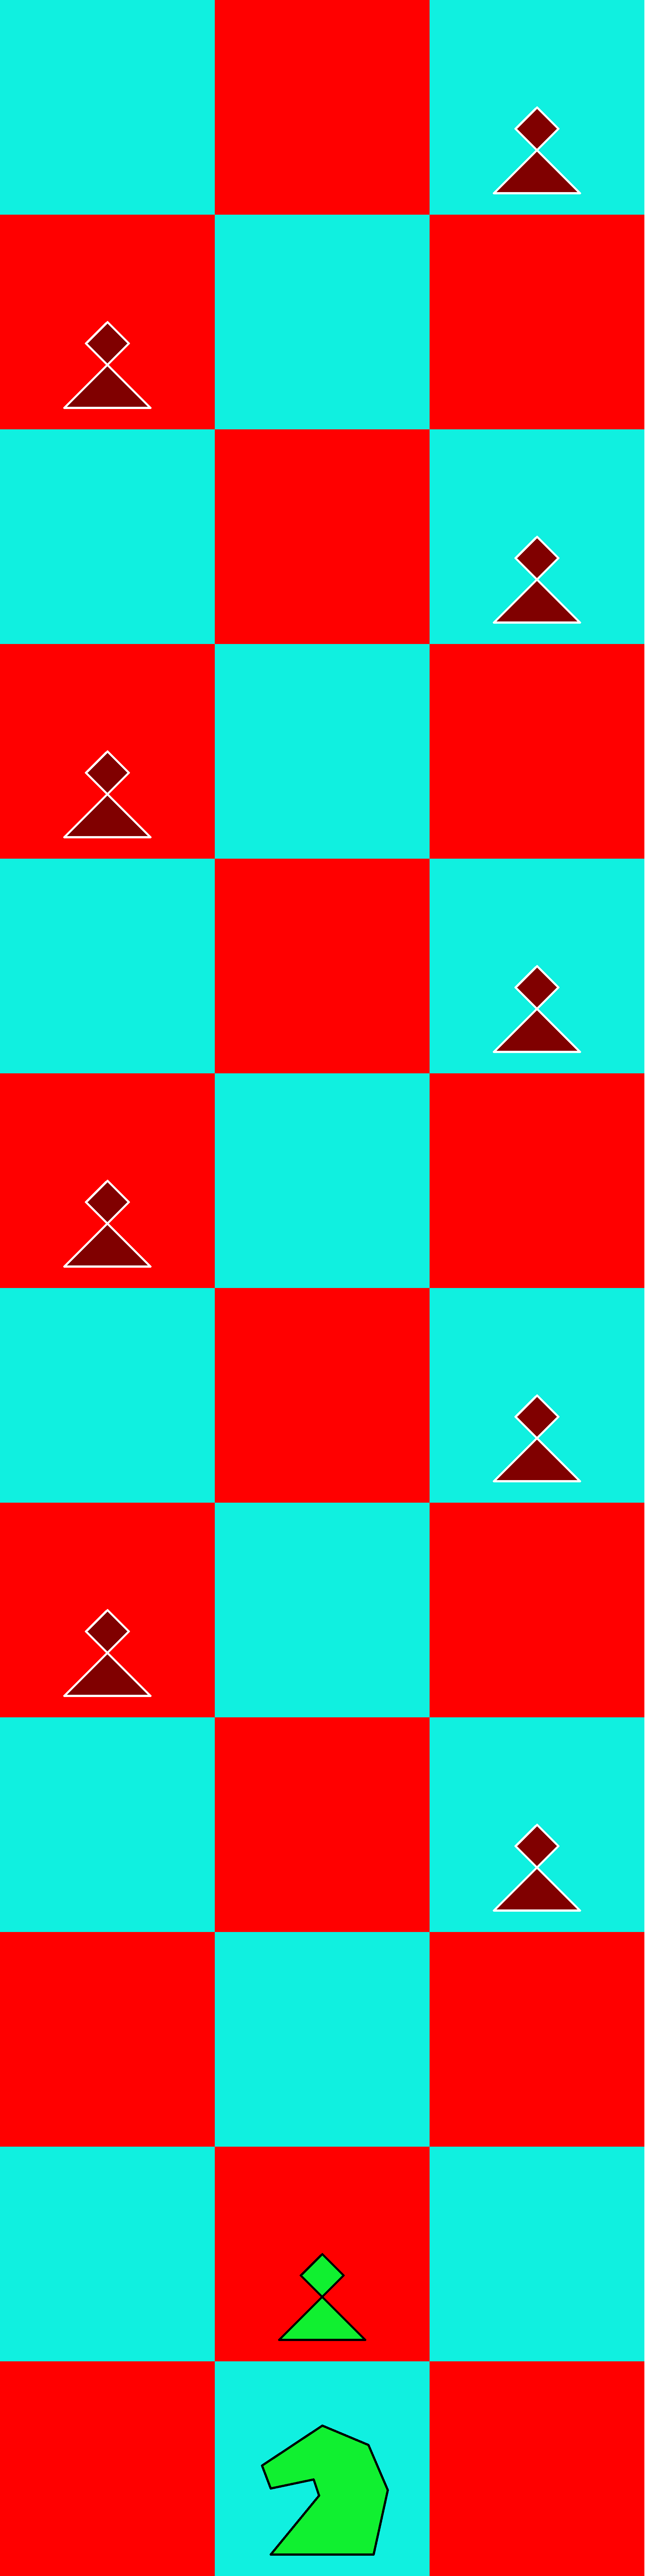
\includegraphics[width=0.125\textwidth, keepaspectratio=true]{en_passants/18_conquest_of_tlalocan_en_passant.png}
\caption{En passant}
\label{fig:18_conquest_of_tlalocan_en_passant}
\end{wrapfigure}
Rush and en passant are identical to those in Classic Chess, only difference
is that Pawn can now move longer on initial turn, up to 9 fields in this
variant.

\clearpage % ..........................................................

\section*{Castling}
\addcontentsline{toc}{section}{Castling}

Castling is the same as in Classical Chess, only difference is that King can move between 2 and 9 fields across.
All other constraints from Classical Chess still applies.

\noindent
\begin{figure}[!h]
% \begin{figure}[!t]
\includegraphics[width=1.0\textwidth, keepaspectratio=true]{castlings/18_cot/conquest_of_tlalocan_castling.png}
\caption{Castling}
\label{fig:conquest_of_tlalocan_castling}
% \centering
\end{figure}

In example above, all valid King's castling moves are numbered.

\noindent
\begin{figure}[!h]
% \begin{figure}[!t]
\includegraphics[width=1.0\textwidth, keepaspectratio=true]{castlings/18_cot/conquest_of_tlalocan_castling_right_08.png}
\caption{Castling long right}
\label{fig:conquest_of_tlalocan_castling_right_08}
% \centering
\end{figure}

In this example King was castling long to the right. Initial King's position is marked with "K".
After castling is finished, right Rook ends up at field immediately left to the King.

\clearpage % ..........................................................

\section*{Initial setup}
\addcontentsline{toc}{section}{Initial setup}

Compared to initial setup of Tamoanchan Revisited, Shaman is inserted between Unicorn and Pyramid
symmetrically, on both sides of chessboard. This can be seen in the image below:

\noindent
% \begin{figure}[t]
\begin{figure}[h]
\includegraphics[width=1.0\textwidth, keepaspectratio=true]{boards/18_conquest_of_tlalocan.png}
\caption{Conquest of Tlalocan board}
\label{fig:18_conquest_of_tlalocan}
% \centering
\end{figure}

\clearpage % ..........................................................
% ======================================== Conquest of Tlalocan chapter
